In the first chapter, theoretical foundations are described. Firstly, terms such as BPM, Business Intelligence are explained. Then, the theory of Enterprise Ontology and DEMO methodology follow. In the end, Gantt chart is described, because it is used as part of visualisation approach. 

\section{Business Process Management}
\gls{bpm} is an approach that focuses on modelling, analysing, improving and monitoring business processes. 
The \gls{bpm} life-cycle can be divided to five stages as shown in \cref{fig:bpm-lifecycle}:

\begin{figure}[ht!]
	\centering
    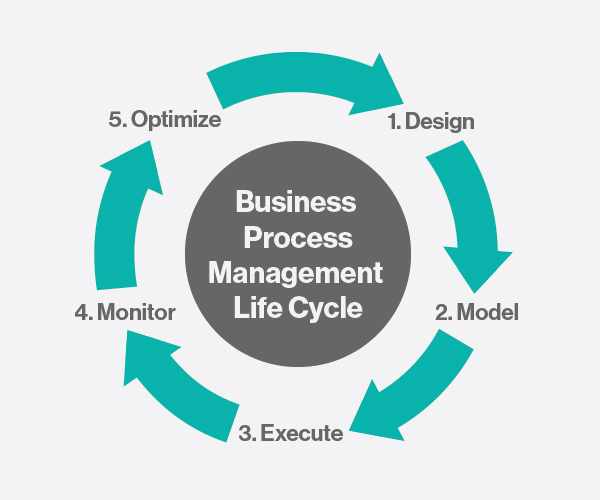
\includegraphics[width=0.6\textwidth, keepaspectratio]{img/bpm-lifecycle.jpg}
    \caption{BPM Life-cycle\cite{harvey-koeppel-bpm-lifecycle-2015}}
    \label{fig:bpm-lifecycle}
\end{figure}

\begin{description}
	\item[Design] The requirements of the business are collected, analysed and specified. The specification can be ``as is'' (state of how processes currently are) or ``to be'' (how processes would be). Accompanying graphical materials (such as flow-charts) are included.
    \item[Model] Specification is expressed (modelled) with graphical notation \gls{bpmn}, which will be investigated later.
    \item[Execute] Changes are implemented and deployed.
    \item[Monitor] After deployed changes, monitoring system comes to the scene. Processes are monitored and \gls{bpms} tools are used to collect data and analyse performance through metrics - called \gls{kpi}. \gls{kpi} are defined, optimized metrics which help to understand the performance of the current business. As an example of \gls{kpi} can be ``an average number of requests for new order per day'' and many more, individual metrics to concrete business.
    \item[Optimize] At some point, when an appropriate number of data are collected and analysed with monitoring, optimization is done. The goal of optimization is to find issues or some improvements. After that, new specifications and improvements are created and \textit{design} stage is executed again.
\end{description}

\todo{Some conclusion about BPM?}

\subsection{Business Process Model and Notation}
\gls{bpmn} is notation created and standardised by \textit{Object Management Group} (see \url{https://www.omg.org}). According to\cite{bpmn-org-2018} \gls{bpmn} can be described as:
\begin{quote}
  \gls{bpmn} is a graphical notation that depicts the steps in a business process. BPMN depicts the end to end flow of a business process. The notation has been specifically designed to coordinate the sequence of processes and the messages that flow between different process participants in a related set of activities.
\end{quote}
The notation itself, elements which are used and how modelling is done, are not described. For this information, see\cite{bpmn-org-2018}.

\section{Business Intelligence}

\gls{bi} is a way how business can collect an enormous amount of data, structure them and analyse (see \cref{fig:bi-diagram}. From \gls{bpm} life-cycle view, \gls{bi} is a \textit{Monitor} stage. Systems which are tagged as \gls{bi} tools typically offers some kind of reporting, dashboards and scorecards. 

\begin{figure}[ht!]
	\centering
    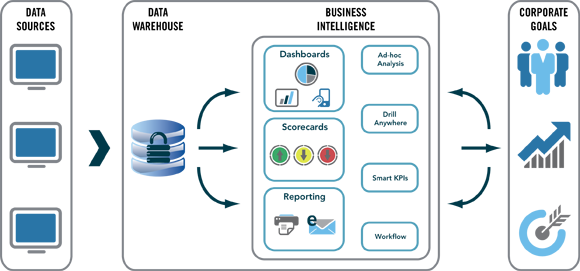
\includegraphics[width=0.6\textwidth]{img/mortgage-business-intelligence-diagram.png}
    \caption{Business intelligence diagram\cite{business-intelligence-diagram-2018}}
    \label{fig:bi-diagram}
\end{figure}

\textbf{Dashboard} offers graphical overviews of collected data. Dashboards are typically highly customizable and can offer different types of views for each employee to help achieve their job. Dashboards can help understand and find issues within business and potentially more quickly solve them. \cref{fig:bi-dashboard} shows an example. \todo{citation of MS POWER BI?}

\textbf{Scorecards} offer monitoring of \gls{kpi} metrics and user can easy compare goals and current results. Scorecards also easily show performance of business, for example if business plan is fulfilled or financial flow (e.g if business is profiting or not,\dots). 

\begin{figure}[ht!]
	\centering
    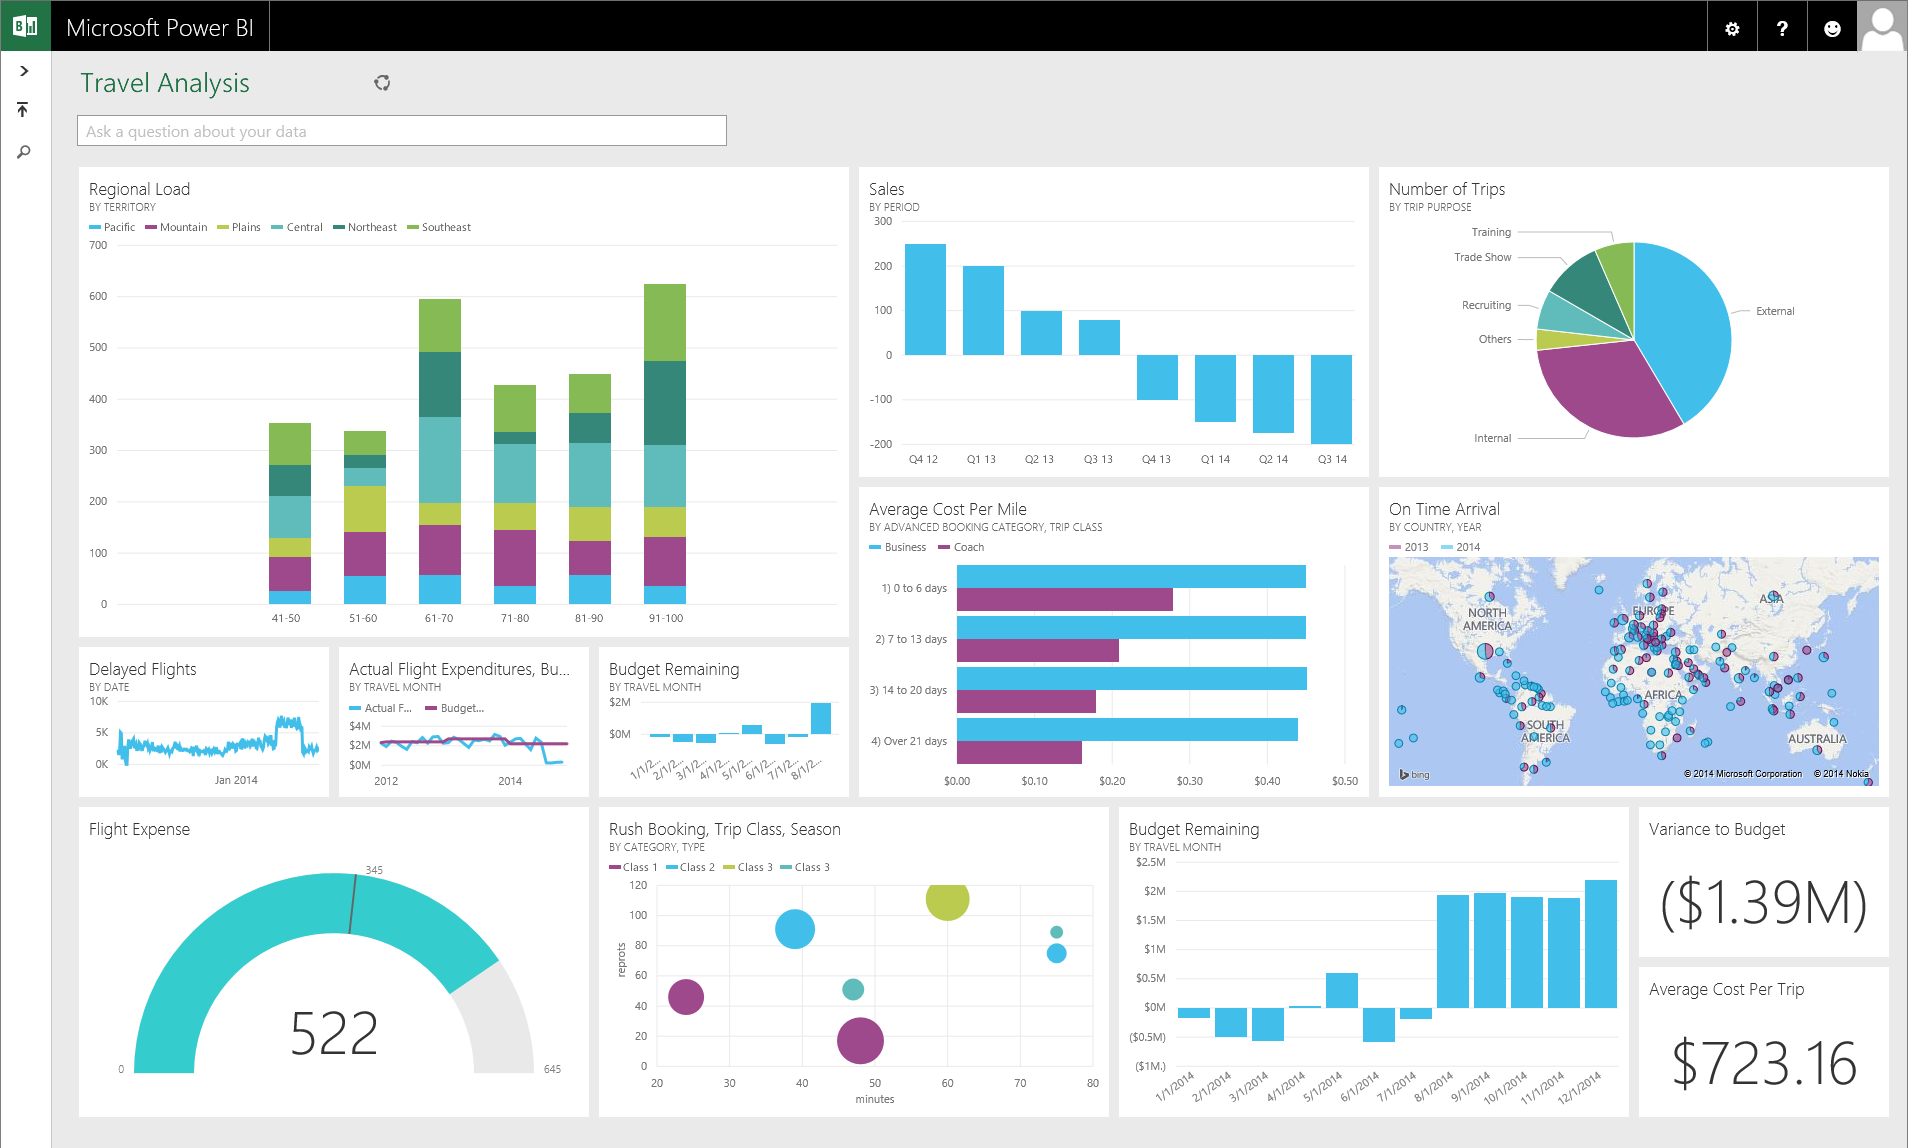
\includegraphics[width=0.6\textwidth]{img/microsoft-power-bi-dashboard.png}
    \caption{Business Intelligence dashboard example\cite{ms-business-intelligence-2018}}
    \label{fig:bi-dashboard}
\end{figure}

\section{Enterprise ontology}
According to\cite{gruber-translation-1993}, definition of ontology states as ``An ontology is a specification of a conceptualization''. In other words ontology is description, a formal specification, of concepts and relationships.

Enterprise Ontology\cite{dietz-essence-2015} is the understanding of the essence of organisation, completely independent of the way in which this essence is realised and implemented.

The DEMO Methodology\cite{dietz-enterprise-2006} is an engineering methodology, based on theory of enterprise ontology.

The following text was taken from article describing \gls{eo} theory\cite{haan-modeling-2009}:

\begin{quotation}
Enterprise ontology is focused on the essence of the operation of an organization, meaning that it is fully independent of the (current) realization and implementation of the organization. The theory that underlies the notion of enterprise ontology as presented by Dietz is called the PSI-theory. Dietz uses this theory to construct a methodology providing an ontological model of an organization, i.e. a model that is coherent, comprehensive, consistent, and concise, and that only shows the essence of the operation of an organization model. This methodology is called \gls{demo}.

Compared to its implementation model, the ontological model of an enterprise offers a reduction of complexity of over 90\%. This reduction of complexity makes an organization for a manager intellectual manageable and transparent. It also shows the coherence between all fields within the enterprise, like business processes, workflow, organization structure, etc.

The overall goal of the PSI-theory (the theory behind the notion of Enterprise Ontology) is to extract the essence of an organization from its actual appearance. It presents four axioms that help to achieve this goal.

The \textbf{operation axiom} (\cref{fig:OperationAxiom}) tells us that the implementation independent essence of an organization is that it consists of subjects fulfilling actor roles. A subject fulfilling a certain actor role is called an actor. Actors constitute the operation of an organization by performing two kinds of acts: production acts and coordination acts.

\begin{figure}[ht!]
	\centering
    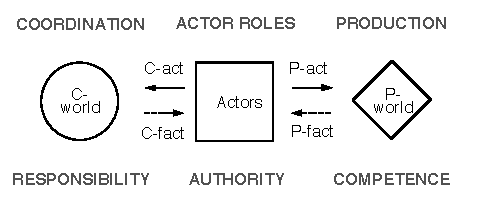
\includegraphics[width=10cm, keepaspectratio]{img/OperationAxiom}
    \caption{The operation axiom\cite{haan-modeling-2009}}
    \label{fig:OperationAxiom}
\end{figure}

By performing production acts (P-acts for short) the subjects contribute to bringing about the goods and/or services that are delivered to the environment of the organization. The results of P-acts are production facts (P-facts for short), which can be divided into material (something is manufactured, stored or transported) and immaterial (decisions or judgements) facts.

By performing coordination acts (C-acts for short) subjects enter into and comply with commitments towards each other regarding the performance of production acts. A C-act is performed by one actor, the performer, and directed to another actor, the addressee. C-acts consist of an intention (e.g. request, promise, question, assertion) and a proposition (the performer proclaims the fact and the associated time the intention is about) and result in coordination facts (C-facts for short).

The \textbf{transaction axiom} tells us that C-acts are performed as steps in universal patterns, called transactions. This axiom reveals universal socionomic patterns of coordination that hold for all organizations. The standard transaction pattern is shown in~ \cref{fig:TransactionPattern}. A white box represents a C-act type and a white disk represents a C-fact type. A gray box represents a P-act type and a gray diamond a P-fact type. 

\begin{figure}[ht!] 
	\centering
    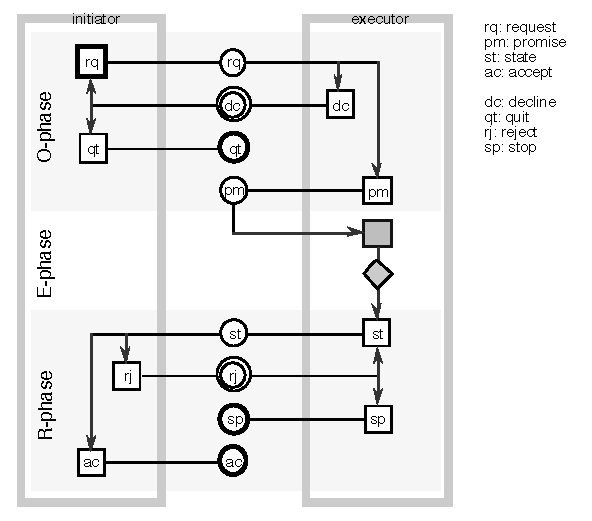
\includegraphics[width=8cm, keepaspectratio]{img/TransactionPattern}    
    \caption{The standard transaction pattern\cite{haan-modeling-2009}}
    \label{fig:TransactionPattern}
\end{figure}

Two actors are involved in a transaction, the initiator and the executor. A transaction evolves in three phases: the order phase (O-phase for short), the execution phase (E-phase for short), and the result phase (R-phase for short).

The \textbf{composition axiom} tells us how P-facts are interrelated. It states that every transaction is enclosed in some other transaction, or is a customer transaction of the organization under consideration, or is a self-activation transaction. According to Dietz this axiom provides the basis for a well-founded definition of the notion of business process.

The \textbf{distinction axiom} (\cref{fig:DisctinctionAxiom}) tells us that actors exert three basic human abilities: performa, informa, and forma. Through the distinction axiom a substantial reduction of complexity and diversity is achieved, regarding both the coordination and the production in an organization.

\begin{figure}[ht!]
	\centering
    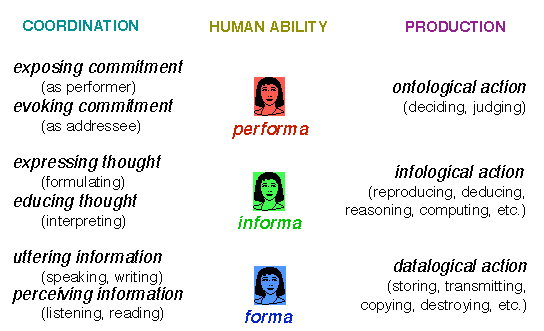
\includegraphics[width=10cm, keepaspectratio]{img/DistinctionAxiom}
    \caption{The distinction axiom\cite{haan-modeling-2009}}
    \label{fig:DisctinctionAxiom}
\end{figure}

\subsection{The Organization Theorem}

The organization theorem combines the benefits of these axioms into one concise, comprehensive, coherent, and consistent notion of enterprise. This theorem states that the organization of an enterprise is a heterogeneous system that is constituted as the layered integration of three homogeneous systems: the B-organization (from Business), the I-organization (from Intellect), and the D-organization (from Document). Figure~ \ref{fig:OrganizationPyramid} visualizes the organization theorem and shows us that the D-organization supports the I-organization, which supports the B-organization. The coordination parts of these three systems are similar, they only differ in the kind of production: the production of the B-organization is ontological, the production in the I-organization is infological, and the production in the D-organization is datalogical.

\begin{figure}[ht!]
	\centering
    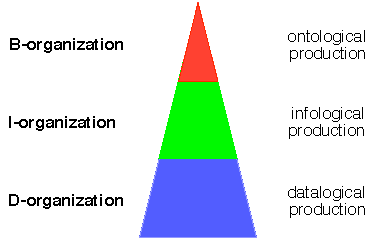
\includegraphics[width=6cm, keepaspectratio]{img/OrganizationPyramid}
    \caption{The organization theorem\cite{haan-modeling-2009}}
    \label{fig:OrganizationPyramid}
\end{figure}

\end{quotation}

\section{Modelling with DEMO}
In this section, firstly short description of modelling aspects is provided and then a illustrative example how modelling with \gls{demo} can be more precise and shorter than creating model with \gls{bpmn}. 

All used elements in DEMO modelling are described in aspects models arranged as pyramid. However the two core elements are Ontological transaction and Actor roles. Good summarization of these two core elements are from master thesis by Zuzana Vejrazkova~\cite{vejrazkova-demo-2013}:

\begin{quote}
	\begin{description}
		\item[Ontological transaction] involves actions that happen on the ontological level, as described by the Distinction axiom. Those involve bringing about the facts that did not exist before, making decisions, or transporting physical elements. Completion of a transaction, in a way that is described by the transaction axiom, results in a new original fact, called the P-fact.
        \item[Actor role] There are two actor roles, the initiator and the executor. They play an important role in DEMO modelling, as each transaction needs to have exactly one initiator and one executor. On the implementation level, 1~person can (and often does) posses more actor roles.
	\end{description}
\end{quote}

Figure \ref{fig:DemoAspectModels} shows that ontological model can be divided to four sub-models. The good and brief explanation is in the book \textit{The essence of organisation: an introduction to enterprise engineering}~\cite{dietz-essence-2015}:

\begin{figure}[ht!]
	\centering
    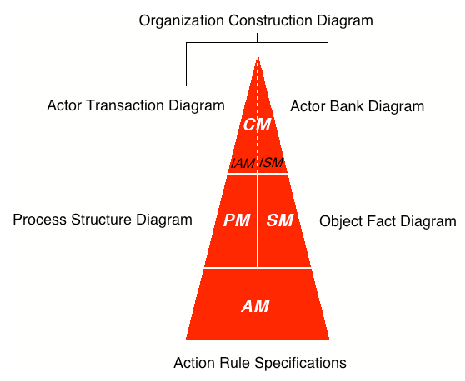
\includegraphics[width=8cm, keepaspectratio]{img/DemoAspectModels}
    \caption{The DEMO Aspect Models pyramid\cite{dietz-discipline-2013}}
    \label{fig:DemoAspectModels}
\end{figure}

\begin{quote}
	\begin{description}
		\item[Construction model] (CM) is the most concise sub-model. Therefore it is put at the top of the triangle. An additional meaning of this position is that there is nothing ``above'' the CM. The Construction Model shows the identified transaction kinds, the corresponding actor roles, and the border of the Scope of Interest.
         \item[Action model] (AM) is the most comprehensive one, in the sense that the other three may be derived from it. The AM of an organisation consists of the action rule specifications for every internal actor role. Action rules are guidelines for dealing with the events that actors have to respond to.         
         \item[Process Model] (PM) shows precisely how the identified transactions are interrelated in tree structures. These tree structures are what people commonly refer to as business process models.         
         \item[Fact Model] (FM) show the fact kinds in the production world of the organisation and their interrelationships. 
	\end{description}
\end{quote}

\begin{figure}[ht!]
	\centering
    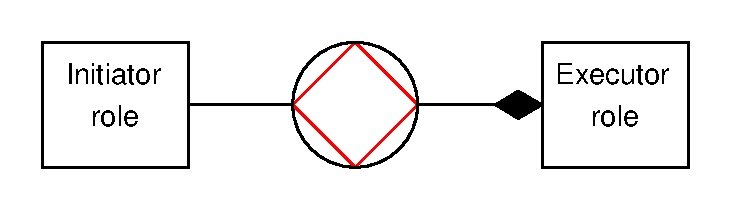
\includegraphics[width=6cm, keepaspectratio]{img/ocd-symbol-example}
    \caption{The core OCD element - transaction symbol with assigned actor roles}
    \label{fig:ocd-symbol-example}
\end{figure}

The PM is in between CM and the AM, that means it is more detailed than CM but less than AM. The PM and the FM are on the same layer of the pyramid and it refers to the fact, that PM takes the process view of coordination world, and the FM is for the production world in the same meaning as PM.

From the CM is used \gls{ocd} which takes standard process pattern and squeeze it to one symbol with two connected boxes which represent initiator and executor actor roles (see \cref{fig:ocd-symbol-example}).

From the PM is taken \gls{psd} sub-model which describes business processes and the exact way how each transaction is connected with another. Following explanation how \gls{psd} is modelled is from~\cite{dietz-essence-2015}:

\begin{quote}
      The disk of the transaction is stretched horizontally, such that it looks like a sausage. One must imagine that there is an invisible and non-proportional time line from left to right (promise is performed after its request,\dots). Coordination acts and facts are represented by small boxes and disks on the border of the transaction symbol (the sausage). 
      The production act, execute, is represented by a small grey box on the edge of the production symbol. To the left of it is the order phase, and to the right the result phase.
      Between two transactions (the sausages) can be added arrows, either solid or dashed. Solid arrows represent \textit{response links}. Response link means that the act at the arrow point is performed in response to the event at the shaft. Dashed arrow represent \textit{waiting links}. Their meaning is that performing the act at the arrow point must wait for the event at the shaft having occurred. Through ``swim lanes'' the responsibility areas of the actor roles are indicated.
\end{quote}
An example of PSD is shown at \cref{fig:psd-example} which means exactly ``When the transaction T1 (Supply order) is \textit{requested}, as a response, T2 (Tax payment) is also \textit{requested}. After that, T1 can be promised only and only, if T2 is \textit{accepted}. After that T1 can be completed''.

\begin{figure}[ht!]
	\centering
    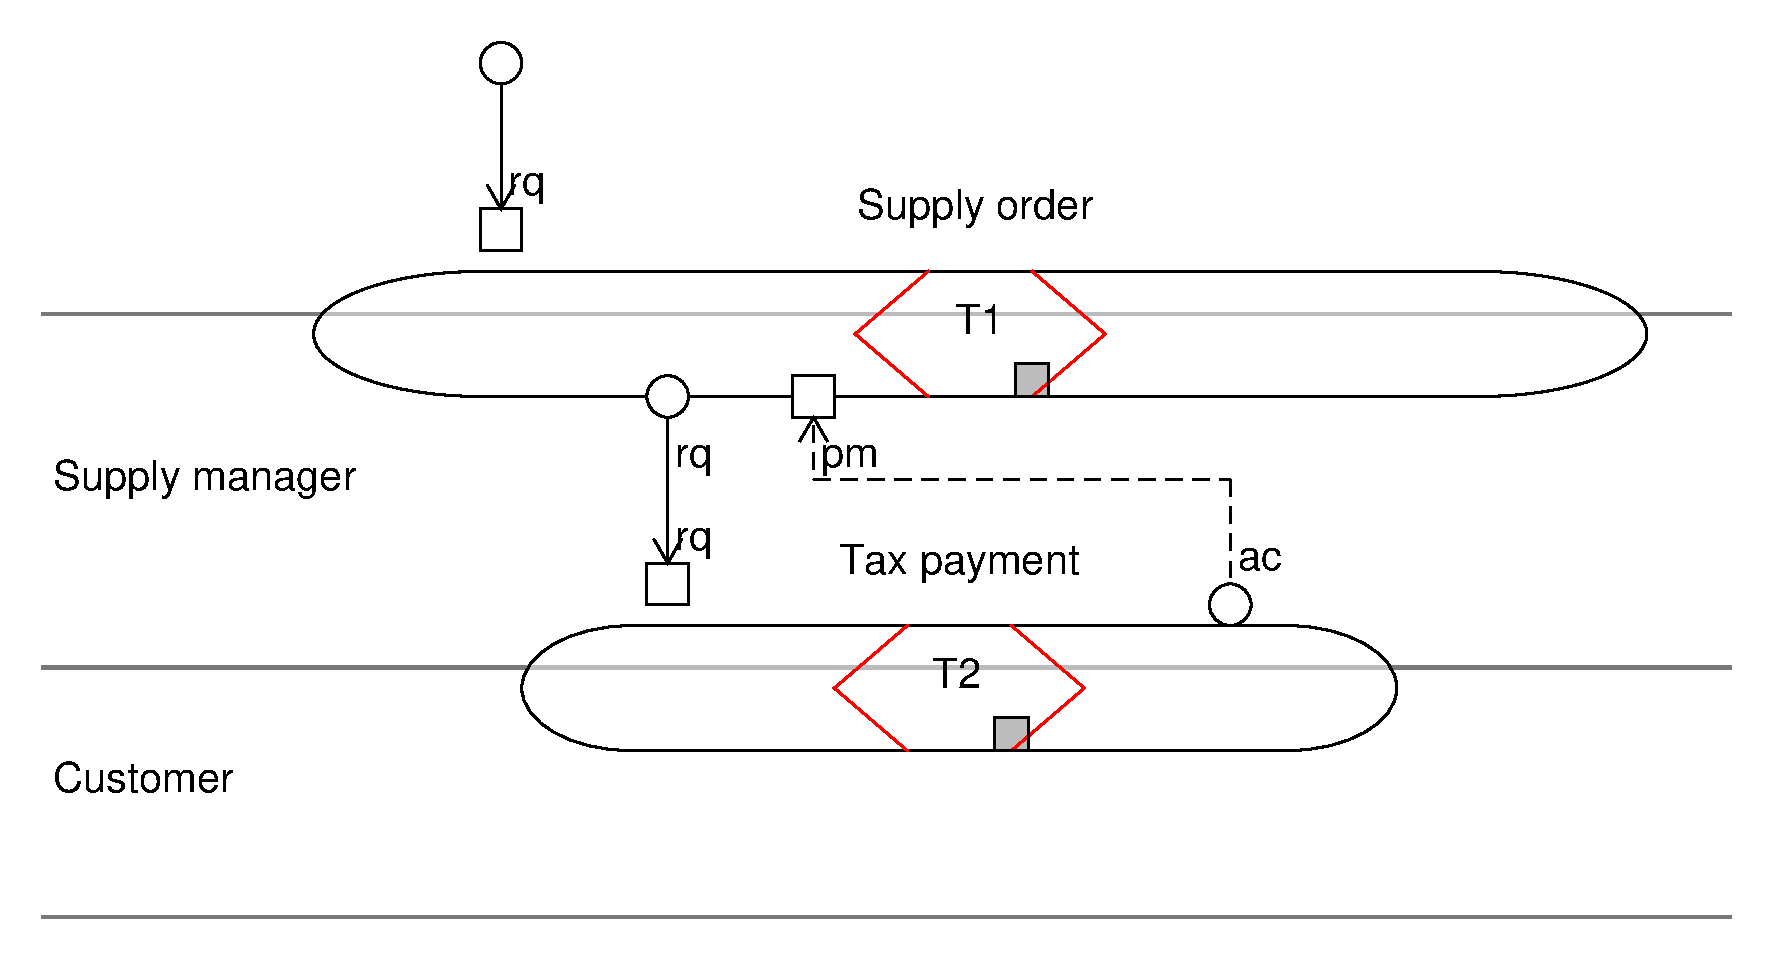
\includegraphics[width=0.7\textwidth]{img/psd-example}
    \caption{PSD example}
    \label{fig:psd-example}
\end{figure}

\subsection{Advantage of DEMO Over BPMN}
    
\gls{bpm} notation is well defined, established and widely used. Many \gls{bpms} exists around and of course, \gls{bpmn} is used ``under the hood''. These systems will be described later in \cref{ch:bpms}.
    
One thing is very clear, with enlarging business requirements, the business processes "grow up" too and so \gls{bpmn} diagrams. This can lead to very large and complex diagrams, which can be harder to read and understand. One of the advantages of DEMO is fact, that same \gls{bpmn} diagram can be represented within DEMO notation. The result is reduced complexity with the same understanding as diagram within \gls{bpmn}. However, advantages of DEMO notation can be used not only within \gls{bpmn}. For example, students at subject MI-MEP (Modelling economic processes, translated) at \gls{ctu}\cite{ccmi-2018} transferred large Trump's flow chart\cite{quartz-trump-2017} (about highway building process) to DEMO OCD diagram. The flow chart that fills several pages, \gls{demo}'s \gls{ocd} fills only one page of size A4. 
To summarize, DEMO can really help to better understand business processes without too much complexity of diagrams itself.

\section{Gantt chart}
According to \cite{gantt-chart-2018}, Gantt chart was proposed in 1890 by Karol Adamiecki, but he did publish his work only in the Polish language. About the year 1910 American engineer, Henry Gantt, introduced his own version of this chart and this work became widely used and is still used by project managers. 
Gantt chart serves as an overview of activities according to the time schedule. By simplicity, Gantt chart shows, what has to be done (an activity) and when.
At \cref{fig:gantt-chart-example} is an example of Gantt chart. The core element is some kind of bar chart (progress bar) which starts at some time and is scheduled to end in some another time.
Nowadays, Gantt charts, has more advanced elements, such as connected activities (one activity must end before another can start), groups of activities, different colours of activities that can indicate different phases of completion and so on. Many systems for time-management support these types of graphs.
Gantt chart and its usage for this thesis are discussed later, in chapter \cref{ch:proposed-approach}.

\begin{figure}[ht!]
	\centering
    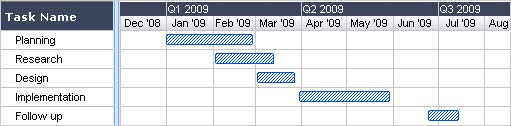
\includegraphics[width=0.8\textwidth]{img/gantt-chart-example.jpg}
    \caption{Gantt chart example\cite{gantt-chart-2018}}
    \label{fig:gantt-chart-example}
\end{figure}

